\documentclass[aspectratio=169]{beamer}

\usepackage[utf8]{inputenc}
\usepackage{amsmath}
\usepackage{amsfonts}
\usepackage{amssymb}
\usepackage{graphicx}
\usepackage{ragged2e}  % `\justifying` text
\usepackage{booktabs}  % Tables
\usepackage{tabularx}
\usepackage{tikz}      % Diagrams
\usetikzlibrary{calc, shapes, backgrounds}
\usepackage{amsmath}
\usepackage{amssymb}
\usepackage{dsfont}
\usepackage{url}       % `\url
\usepackage{listings}  % Code listings
\usepackage[T1]{fontenc}
\usepackage[backend=biber, style=ieee, citestyle=numeric-comp, isbn=false, url=false, doi=false, giveninits=true, uniquename=init]{biblatex}
\usepackage{hyperref}
\usepackage{caption}
\usepackage{theme/beamerthemehbrs}
\addbibresource{rnd.bib} % Your bibliography file
\newcommand\blfootnote[1]{%
  \begingroup
  \renewcommand\thefootnote{}\footnote{#1}%
  \addtocounter{footnote}{-1}%
  \endgroup
}


\author[Shinas Shaji]{Shinas Shaji}
\title{Evaluation of Few-Shot Transfer of Vision-Language Foundation Models to Learn Lightweight Models for Robotic Vision Tasks}
\subtitle{R\&D Project Defense}
\institute[HBRS]{Hochschule Bonn-Rhein-Sieg}
\date{\today}
\subject{R\&D Project Defense}

% leave the value of this argument empty if the advisors
% should not be included on the title slide
\def\advisors{Prof. Dr. Sebastian Houben (H-BRS, Fraunhofer IAIS), \\
Santosh Thoduka M.Sc. (Fraunhofer IAIS)}

% \thirdpartylogo{path/to/your/image}


\begin{document}
{
\begin{frame}
\titlepage
\end{frame}
}


\section{Introduction}
\begin{frame}{Introduction}
\framesubtitle{Vision-Language Models (VLMs)}
  \begin{itemize}
    \item Neural networks that process both \emph{images} and \emph{text}
    \item Like Large Language Models (LLMs):
    \begin{itemize}
      \item Learn \emph{general visual-textual understanding} from pre-training~\footfullciteieee{Radford2021}
      \item Then aligned to human preferences and \emph{instruction-following}
    \end{itemize}
    \item Shown to be able to \emph{adapt} to new tasks without extensive task-specific training~\footfullciteieee{Liu2023}, hence quite \emph{generalizable}
    \blfootnote{\vspace{0.05em}}
  \end{itemize}
\end{frame}
% SPEAKER NOTES: 
% - VLMs combine computer vision and natural language processing capabilities in a single neural network
% - Pre-training occurs on millions of image-text pairs from the web (e.g., CLIP was trained on 400M image-text pairs)
% - Unlike traditional CV models trained for specific tasks, VLMs learn broader understanding that transfers to many tasks
% - Similar to how ChatGPT can answer questions on many topics, VLMs can handle multiple visual tasks


\begin{frame}{Introduction}
\framesubtitle{Few-Shot Transfer}
  \begin{itemize}
    \item Teaching a \emph{generalizable model} new tasks by showing it a few \emph{examples}
    \item Model `learns' to recognize patterns from these examples
    \item Can then apply this `learning' to new, unseen instances
  \end{itemize}
  \begin{columns}[onlytextwidth]
    \column{.5\textwidth}
    % \centering 
    \small{\emph{Prompt}: A [DOG] has droopy ears and is often fluffy. This is a [DOG]:}
    \begin{figure}
      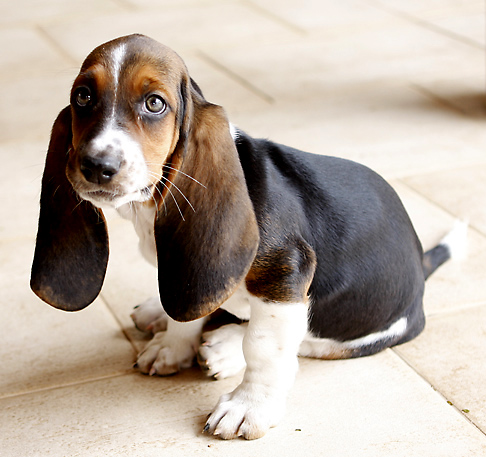
\includegraphics[width=20mm]{./figures/basset-hound.jpeg}
      \caption{\centering This is a [DOG]. \\ \tiny{Image from Wikipedia, \href{https://commons.wikimedia.org/w/index.php?curid=32270218}{Link}}}
    \end{figure}
    \column{.5\textwidth} 
    \begin{figure}
      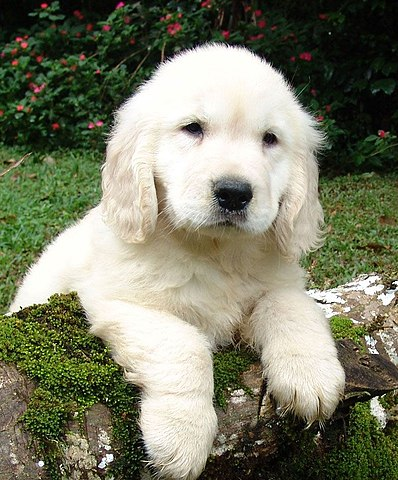
\includegraphics[width=20mm]{./figures/golden-retriever-puppy.jpeg}
      \caption{\centering Is this a [DOG]? \\ \tiny{Image from Wikipedia, \href{https://commons.wikimedia.org/w/index.php?curid=18521767}{Link}}}
    \end{figure}
    \vspace{-0.4cm}
    % \centering 
    \small{\emph{Prompt}: Is this a [DOG]?\\
    \emph{Expected Answer}: Yes}
  \end{columns}
\end{frame}
% SPEAKER NOTES:
% - Few-shot transfer is different from traditional machine learning that requires many examples
% - The model doesn't actually learn in the traditional sense; it leverages knowledge from pre-training
% - In this example, we show the model one example of a dog (a basset hound) and ask it to identify another dog
% - This works because the model already knows what dogs look like from pre-training
% - The quotation marks around 'learns' emphasize that it's not learning from scratch. I like to think of it as somehow narrowing the tree of possible responses from a point.


\subsection{Motivation}
\begin{frame}{Motivation}
  \framesubtitle{Few-Shot Transfer}
  \begin{columns}[T]
    \column{0.5\textwidth}
      \centering \emph{Fine-tuning}
      \begin{itemize}
        \item Requires significant computational resources, modifies model parameters
        \item Needs \emph{large amounts} of \emph{labeled data}
        \item Can lead to catastrophic forgetting
        \item Refers to fine-tuning a pre-trained/instruction-tuned model on a specific task
      \end{itemize}
    \column{0.5\textwidth}
    \centering \emph{Few-shot Transfer}
    \begin{itemize}
        \item Uses \emph{`few' examples} or natural language \emph{descriptions}
        \item No model parameters are updated
        \item Potentially more practical for real-world applications~\footfullciteieee{Brown2020}
        \item Can be less effective for complex tasks
    \end{itemize}
  \end{columns}
\end{frame}
% SPEAKER NOTES:
% - Fine-tuning is the traditional approach for adapting pre-trained models to new tasks
% - For VLMs, fine-tuning can require multiple high-end GPUs and days of compute time
% - Catastrophic forgetting means the model may lose previously learned capabilities
% - Few-shot transfer is much more efficient - we can use the model "as is"
% - An important distinction: fine-tuning modifies the model weights, few-shot transfer doesn't
% - The trade-off is that few-shot performance may not match fine-tuned performance for complex tasks


\subsection{Problem Statement}
\begin{frame}{Problem Statement}
\framesubtitle{Dataset Labeling for Computer Vision Tasks}
  \textbf{Challenge:} Creating labeled datasets to train specialized models for computer vision tasks is \emph{time-consuming} and \emph{expensive}~\footfullciteieee{Deng2009}, but VLMs are generalizable
  \vspace{0.5em}

  \textbf{Constraint:} However, VLMs are too \emph{computationally intensive} for direct deployment on resource-constrained environments (e.g., robots)
  \vspace{0.5em}
    
  \textbf{Opportunity:} VLMs could potentially automate label generation (\emph{pseudolabels}) to train \emph{downstream} models
  \vspace{2em}

  \centering \textbf{Research Question:} Can VLMs be transferred to generate \emph{pseudolabels} for computer vision tasks to train \emph{lightweight} downstream models?
  \blfootnote{\vspace{0.05em}}
\end{frame}
% SPEAKER NOTES:
% - The annotation of the ImageNet dataset required crowdsourcing to be feasible
% - Specialized datasets like medical imaging can be even more expensive and require expert annotators
% - VLMs require significant computational resources - multiple high-end GPUs with significant amounts of memory
% - Most robots have limited computational capabilities - often a single low-power GPU or CPU
% - Pseudolabels are automatically generated annotations that can be used in place of human-created labels
% - The key insight: we don't need to deploy the large model - we use it to train a smaller, more efficient model


% \subsection{Proposed Approach}
\begin{frame}{Proposed Approach}
\framesubtitle{Evaluating VLMs for Pseudolabel Generation}
  \textbf{Approach:} Evaluate VLMs on generating \emph{accurate pseudolabels} under various \emph{zero-shot} and \emph{few-shot} transfer conditions
  \vspace{0.3em}
    
  \begin{columns}[T]
    \column{0.55\textwidth}
      \centering \textbf{Key Research Aspects}
      \begin{enumerate}
        \item How does the \emph{number of examples} (few-shot vs. zero-shot) affect pseudolabel quality?
        \item What are the \emph{computational requirements} for practical application?
        \item How effective are the \emph{downstream models} trained on pseudolabels?
      \end{enumerate}

    \column{0.45\textwidth}
    \begin{figure}
      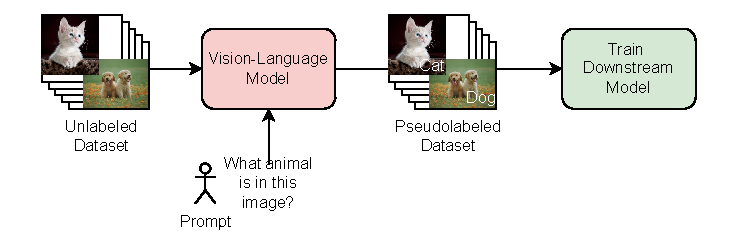
\includegraphics[width=\textwidth]{figures/vlm_transfer_downstream.pdf}
      \caption{\centering Using VLMs to generate pseudolabels for downstream model training}
    \end{figure}
  \end{columns}
\end{frame}
% SPEAKER NOTES:
% - Zero-shot means only describing the task in natural language; few-shot means providing examples
% - We tested multiple prompting strategies to find the most effective approach
% - We examined both common visual tasks (CIFAR-10) and specialized tasks (dermatology) to see if few-shot transfer is generalizable
% - This design helps us understand when VLMs can be reliably transferred for automatic labeling
% - For computational requirements, we measured inference time, memory usage, and scaling properties
% - Downstream models were evaluated against models trained on ground truth labels


\section{Related Work}
\subsection{Vision-Language Models}
\begin{frame}{Related Work}
\framesubtitle{Development of Vision-Language Models}
  \begin{columns}[T]
    \column{0.5\textwidth}
    \begin{itemize}
      \item \emph{Alignment models}: Generate unified text-image embeddings (CLIP~\footfullciteieee{Radford2021}, FLAVA)
      \item \emph{Generative models}: Geneate text conditoined on multimodal inputs (Flamingo, Frozen~\footfullciteieee{Tsimpoukelli2021}, GPT-4o, Claude 3/3.5/3.7, etc.)
    \end{itemize}
    \column{0.5\textwidth}
      \textbf{Architectural Approaches}
      \begin{itemize}
        \item \emph{Towered}: Separate vision and language models with adapters
        \item \emph{Unified}: Single model processing both modalities "early on"~\footfullciteieee{ChameleonTeam2024}
      \end{itemize}
      \vspace{0.3em}
      \textbf{Key Insight}: Enables framing vision tasks as text generation~\footfullciteieee{Cho2021}, enabling streamlined task transfer
  \end{columns}
\end{frame}
% SPEAKER NOTES:
% - Vision-Language Models (VLMs) have progressed significantly since the introduction of CLIP.
% - Alignment models, such as CLIP, are designed to learn joint representations but do not generate textual outputs.
% - In contrast, generative models are capable of producing text responses based on visual inputs.
% - The Frozen model pioneered the approach of freezing the language model (LLM) while solely training the vision encoder.
% - Contemporary VLMs often incorporate separate pre-trained components for vision and language, connected through adapters or connectors.
% - Additionally, unified architectures that process both modalities simultaneously have emerged, enhancing the integration of vision and language tasks.
% - A pivotal advancement facilitating few-shot transfer is the conceptualization of vision tasks as text generation tasks.
% - This paradigm allows us to articulate tasks using natural language, eliminating the need for specialized architectures.
% - The rapid evolution of this field has led to the emergence of models like GPT-4o, which can comprehend and reason about complex visual scenarios.



\subsection{Few-Shot Transfer Learning}
\begin{frame}{Related Work}
\framesubtitle{Transfer Learning \& Adaptation Techniques}
  \begin{columns}[T]
    \column{0.55\textwidth}
      \textbf{Prompting Techniques}
      \begin{itemize}
        \item Crafting prompts to improve task performance~\footfullciteieee{Liu2023}
        \item In-context learning: Providing examples in context~\footfullciteieee{Brown2020}
        \item Chain-of-thought prompting for complex reasoning~\footfullciteieee{Wei2022}
      \end{itemize}
      \vspace{0.5em}
      \textbf{Parameter-Efficient Fine-Tuning}
      \begin{itemize}
        \item Prefix-tuning: Optimizing task-specific prompt vectors~\footfullciteieee{Li2021}
        \item Requires fewer parameters than full fine-tuning
      \end{itemize}
    \column{0.45\textwidth}
      \textbf{Research Gaps}
      \begin{itemize}
        \item Few-shot transfer in VLMs less explored than in NLP
        \item Limited research on VLMs for dataset annotation
        \item Few studies on downstream model performance with VLM-generated labels
        \item Our work addresses these gaps
      \end{itemize}
  \end{columns}
\end{frame}
% SPEAKER NOTES:
% - Prompting techniques are crucial for adapting models to new tasks without retraining
% - In-context learning allows models to learn from examples without parameter updates
% - Chain-of-thought prompting helps models break down complex tasks into simpler steps
% - Parameter-efficient fine-tuning methods like prefix-tuning are valuable for low-resource settings
% - These techniques are less explored in VLMs compared to NLP models
% - Our research contributes by evaluating these methods in the context of VLMs for dataset annotation


\subsection{Applications and Datasets}
\begin{frame}{Related Work}
\framesubtitle{Applications and Datasets}
  \begin{columns}[T]
    \column{0.55\textwidth}
      \textbf{Applications of VLMs}
      \begin{itemize}
        \item Large-scale pre-training enables generalization
        \item Contrast with traditional DNNs trained on specific tasks
      \end{itemize}
      \vspace{0.5em}
      \textbf{Auxiliary Learning Tasks}
      \begin{itemize}
        \item Self-supervised generation of auxiliary labels~\footfullciteieee{Liu2019}
        \item Visual instruction tuning for generative models~\footfullciteieee{Liu2023a}
      \end{itemize}
    \column{0.45\textwidth}
      \textbf{Key Datasets}:
      Various datasets exist for various vision tasks.
      \begin{itemize}
        \item ImageNet, CIFAR-10~\footfullciteieee{Krizhevsky2009}: Object recognition
        \item Microsoft COCO: Detection, segmentation, captioning
        \item Derm7Pt~\footfullciteieee{Kawahara2019}: Specialized dermatology dataset
        \item MVTec: Anomaly detection
      \end{itemize}
  \end{columns}
\end{frame}
% SPEAKER NOTES:
% - VLMs are used in a wide range of vision tasks, leveraging their ability to generalize from large-scale pre-training
% - Traditional DNNs are typically trained on specific datasets for specific tasks, limiting their generalization
% - Auxiliary learning tasks can enhance model performance by providing additional context or training signals
% - Self-supervised methods generate labels without human intervention, reducing the need for manual annotation
% - Key datasets like ImageNet and CIFAR-10 are benchmarks for evaluating model performance on object recognition
% - Specialized datasets like Derm7Pt are crucial for testing models on domain-specific tasks
% - Our research leverages these datasets to evaluate the effectiveness of VLMs in generating pseudolabels for downstream tasks

\section{Methodology}
\subsection{Experimental Setup}
\begin{frame}{Experimental Setup}
    % Content will be added later
\end{frame}

\subsection{Datasets}
\begin{frame}{Datasets}
    % Content will be added later
\end{frame}

\subsection{Models and Prompting Strategies}
\begin{frame}{Models and Prompting Strategies}
    % Content will be added later
\end{frame}

\section{Evaluation}
\subsection{CIFAR-10 Experiments}
\begin{frame}{CIFAR-10 Experiments}
    % Content will be added later
\end{frame}

\subsection{Downstream Model Training}
\begin{frame}{Downstream Model Training}
    % Content will be added later
\end{frame}

\subsection{Specialized Domain (Derm7Pt) Experiments}
\begin{frame}{Specialized Domain Experiments}
    % Content will be added later
\end{frame}

\subsection{Computational Resources Analysis}
\begin{frame}{Computational Resources Analysis}
    % Content will be added later
\end{frame}

\section{Conclusions}
% \subsection{Key Findings}
\begin{frame}{Key Findings}
    % Content will be added later
\end{frame}

% \subsection{Limitations and Future Work}
\begin{frame}{Limitations and Future Work}
    % Content will be added later
\end{frame}

% \section{Q\&A}
\begin{frame}{Thank You!}
    \centering
    \vfill
    {\LARGE Questions?}
    \vfill
    \begin{itemize}
        \item Email: shinas.shaji@smail.inf.h-brs.de
    \end{itemize}
    \vfill
\end{frame}

\end{document}
